\documentclass[11pt]{report}
\usepackage{geometry}                % See geometry.pdf to learn the layout options. There are lots.
\geometry{letterpaper}                   % ... or a4paper or a5paper or ... 
%\geometry{landscape}                % Activate for for rotated page geometry
\usepackage[parfill]{parskip}    % Activate to begin paragraphs with an empty line rather than an indent
\usepackage{graphicx}
\usepackage{amssymb}
\usepackage{epstopdf}
\DeclareGraphicsRule{.tif}{png}{.png}{`convert #1 `dirname #1`/`basename #1 .tif`.png}

\title{RaySys User Manual}
\author{Steven Mashmeyer\\CamdenNarzt\\Oscar Ramirez}
%\date{}                                           % Activate to display a given date or no date

\begin{document}
\maketitle

\chapter*{Login}
\begin{figure}[htb]
  \begin{center}
    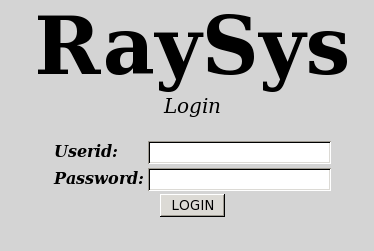
\includegraphics[scale=0.55]{imgs/login.png}
    \caption{RaySys Login}
    \label{fig:login}
  \end{center}
\end{figure}

The system will first present the user with an option to login in. The user should provide a valid userID and password to login.

\chapter*{Header}
Once logged in the first thing the user should notice is how depending on it's user privileges he will be presented with one of the following headers:

\begin{figure}[htb]
  \begin{center}
    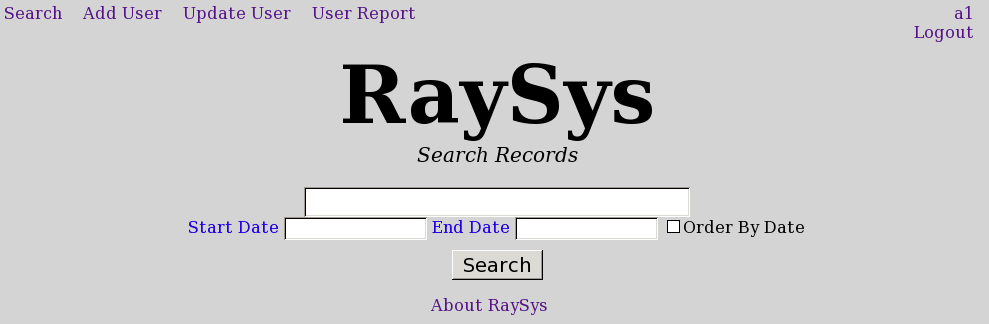
\includegraphics[scale=0.50]{imgs/adminheader.png}
    \caption{Sample Admin header}
    \label{fig:adminh}
  \end{center}
\end{figure}

\begin{figure}[htb]
  \begin{center}
    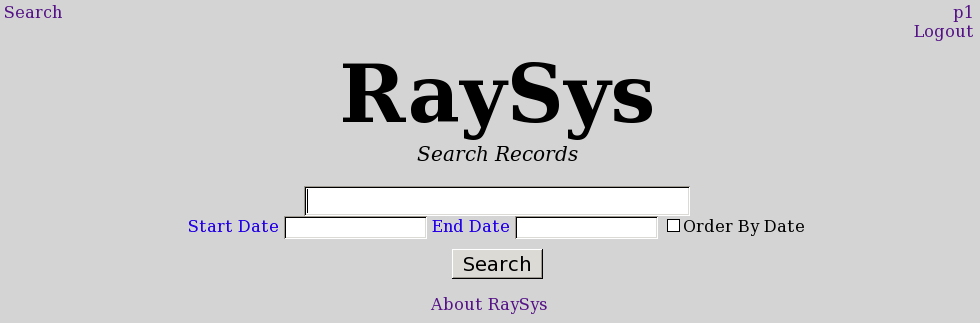
\includegraphics[scale=0.50]{imgs/patientheader.png}
    \caption{Sample Patient header}
    \label{fig:patienth}
  \end{center}
\end{figure}

\begin{figure}[htb]
  \begin{center}
    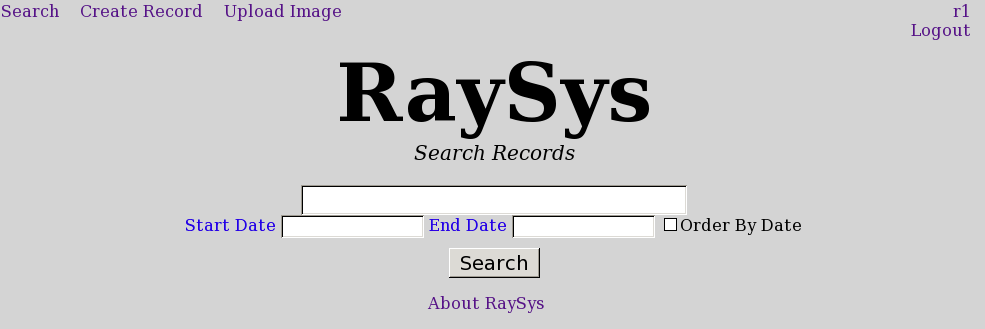
\includegraphics[scale=0.50]{imgs/radioheader.png}
    \caption{Sample Radiologyst header}
    \label{fig:radioh}
  \end{center}
\end{figure}

\begin{figure}[htb]
  \begin{center}
    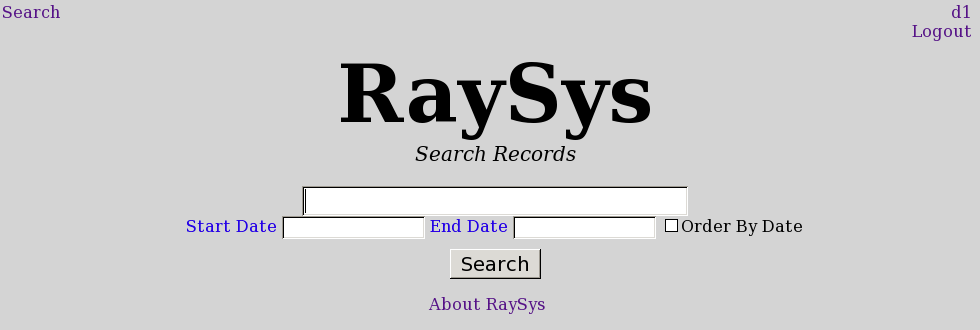
\includegraphics[scale=0.50]{imgs/doctorheader.png}
    \caption{Sample Doctor header}
    \label{fig:doch}
  \end{center}
\end{figure}


\chapter*{Admin}
\section*{Add User}
\begin{figure}[htb]
  \begin{center}
    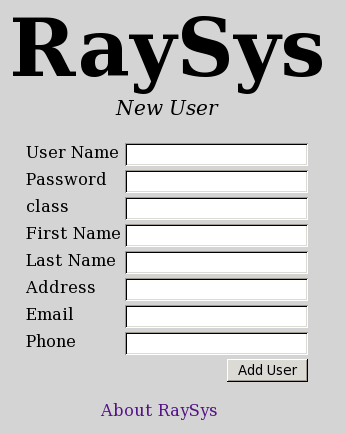
\includegraphics[scale=0.50]{imgs/useradd.png}
    \caption{Sample User Add Screen}
    \label{fig:useraddh}
  \end{center}
\end{figure}

To add a user simply fill in the form with appropriate data and click Add User

\section*{User Update}

\begin{figure}[htb]
  \begin{center}
    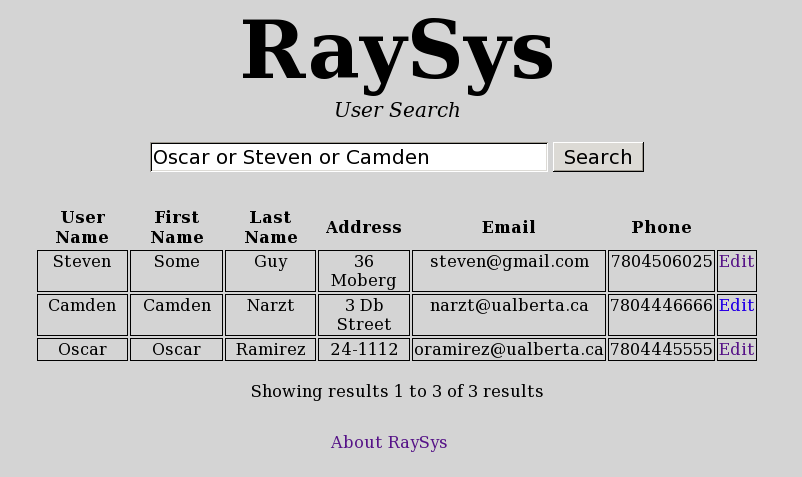
\includegraphics[scale=0.50]{imgs/us1.png}
    \caption{User Update Step 1}
    \label{fig:us1}
  \end{center}
\end{figure}

In order to Update user information simply search for the user names and select which one to edit by clicking the edit hyperlink.

\begin{figure}[htb]
  \begin{center}
    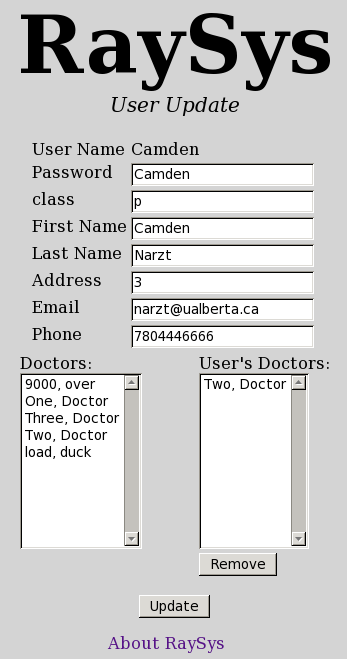
\includegraphics[scale=0.60]{imgs/us2.png}
    \caption{User Update Step 2}
    \label{fig:us2}
  \end{center}
\end{figure}

Once selected simply update the information as needed, click on the desired doctors to be added to the user's set of Doctors and click update. To remove doctors simply select then from the list on the right and click remove. Once you are done updating click the update button.

\section*{Report Generation}
\begin{figure}[htb]
  \begin{center}
    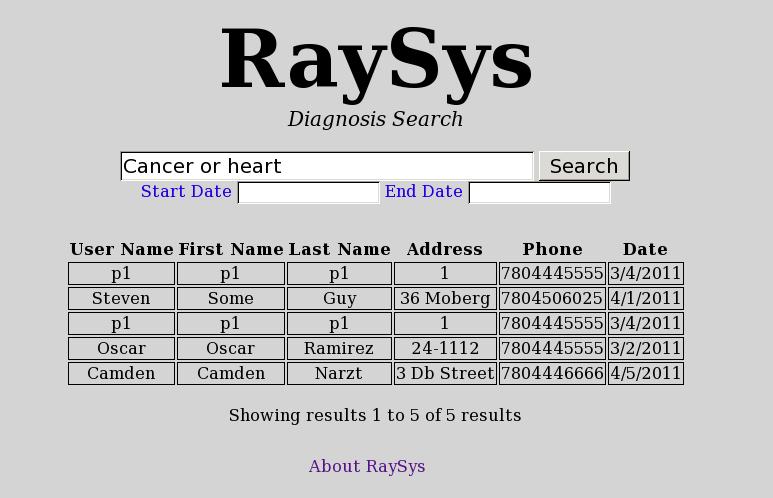
\includegraphics[scale=0.60]{imgs/rg1.png}
    \caption{Report Generation}
    \label{fig:rg1}
  \end{center}
\end{figure}

Report generation is as easy as search, simply input the desired diagnosis to be searched and the date range if needed by clicking on the start date and end date links.

\chapter*{Radiologyst}
\section*{Add Record}
\begin{figure}[htb]
  \begin{center}
    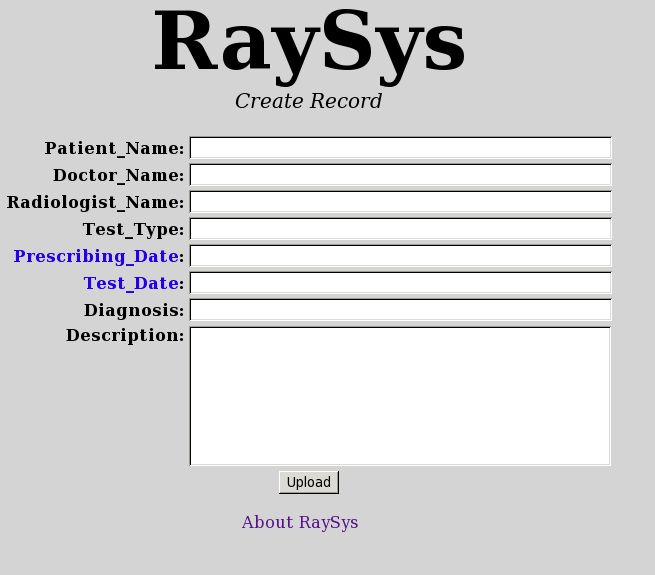
\includegraphics[scale=0.60]{imgs/rad1.png}
    \caption{Radiologyst Record Creation}
    \label{fig:rad1}
  \end{center}
\end{figure}

To create a record simply fill in the form. Note that calendars pop up from the Prescribing and test date links

\section*{Upload Image}
\begin{figure}[htb]
  \begin{center}
    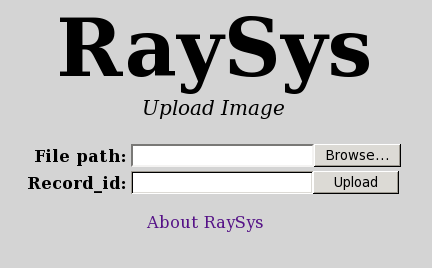
\includegraphics[scale=0.60]{imgs/rad2.png}
    \caption{Radiologyst Upload Image}
    \label{fig:rad2}
  \end{center}
\end{figure}

\chapter*{General Use}
\section*{Search}

\begin{figure}[htb]
  \begin{center}
    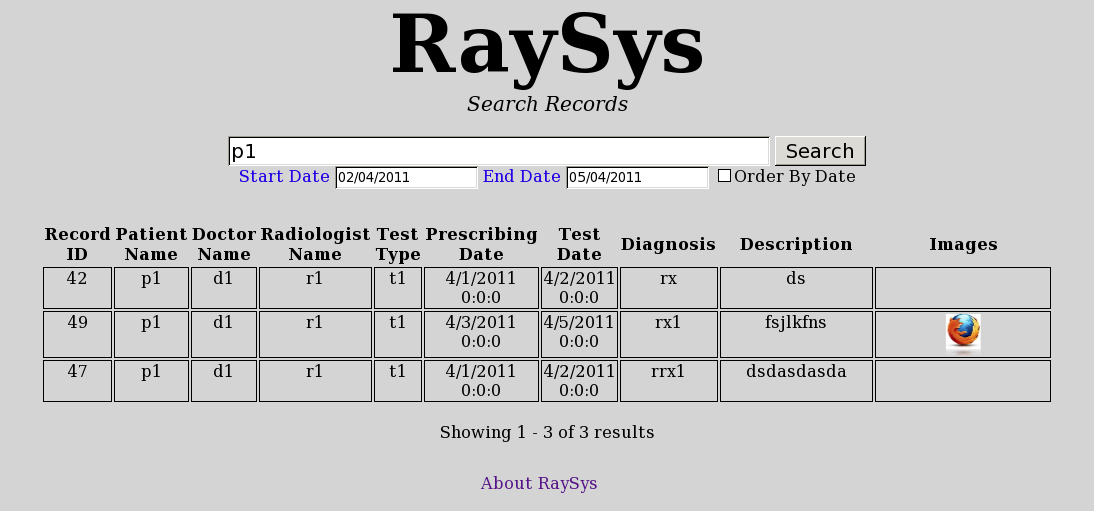
\includegraphics[scale=0.50]{imgs/search1.png}
    \caption{Sample search}
    \label{fig:gen1}
      \end{center}
\end{figure}

Search will display the result information along with the images for that patient, if there are many image simply use your scroll wheel to shift through the images.

\begin{figure}[htb]
  \begin{center}
    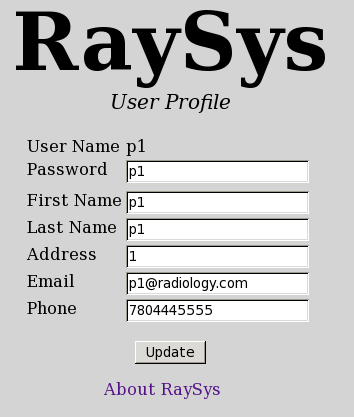
\includegraphics[scale=0.50]{imgs/profile1.png}
    \caption{Update Profile}
    \label{fig:prof1}
    \end{center}
    By clicking on your name you can update your user information
\end{figure}

\end{document}  